\begin{frame}
    \centering
    \begin{figure}[H]
        
\includegraphics[keepaspectratio, width=0.7\paperwidth, height=\paperheight]{LeeLogo}
    \end{figure}
    Informatik: Programmieren\\
    \emoji{abacus} Kapitel 03 (Teil 2): \textbf{Variablen erstellen und verändern}
\end{frame}

% command to make sure colorboxes don't create whitespace between code lines
\fboxsep=.6pt

% default settings for listings
\lstset{style=TigerJython, basicstyle=\scriptsize\ttfamily,escapechar=!}


\begin{frame}[fragile]{Beispiel 3.9: Erstes Programm \emoji{turtle}}
\begin{minipage}[c]{.2\pagewidth}
    \begin{figure}[H]
        \centering
        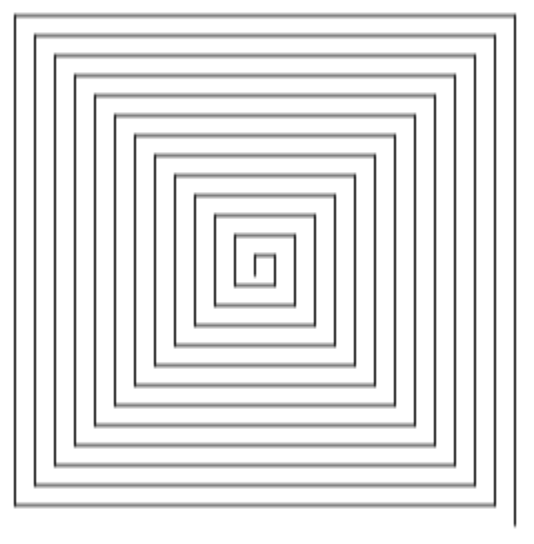
\includegraphics[width=\linewidth,]{GrundlagenInfo/00_Programmieren/Figures/prog-7-spirale.png}
    \end{figure}
    \begin{table}[H]
    \centering
    \hfill
    \scriptsize
    \begin{tabular}{c|c}
         \textbf{Variable} & \textbf{Wert} \\\midrule
         \texttt{seite} & 10 
    \end{tabular}
    \hfill
\end{table}
\end{minipage}\hfill
    \begin{minipage}[c]{.72\linewidth}
    \begin{lstlisting}
from gturtle import *

def spirale(seite):
    forward(seite)
    right(90)
    forward(seite + 5) # erhöhe Seite um 5
    right(90)
    forward(seite + 10) # erhöhe Seite um 10
    right(90)
    forward(seite + 15) # erhöhe Seite um 15
    right(90)
    ...
    forward(seite + 245) # erhöhe Seite um 245
    right(90)

makeTurtle()
spirale(10)    
\end{lstlisting}
\end{minipage}
\begin{itemize}
    \item Die Turtle beginnt in der Mitte. 
    \item Jede Seite ist um 5 länger als die vorherige.
    \item Das Programm ist lang und aufwendig.
    \item Eine \pythoninline{repeat}-Schleife scheint nicht möglich, weil immer eine andere Zahl addiert wird ($5, 10, 15, \ldots, 245$).
\end{itemize}
\end{frame}



\begin{frame}[fragile]{Beispiel 3.9: Zweites Programm \emoji{turtle}}
\begin{minipage}[c]{.2\pagewidth}
    \begin{figure}[H]
        \centering
        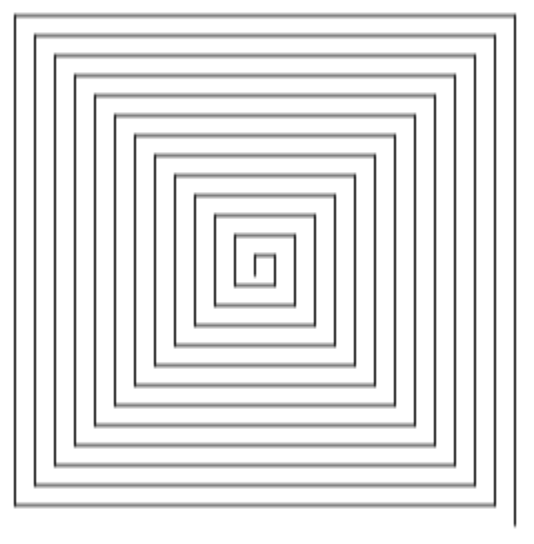
\includegraphics[width=\linewidth,]{GrundlagenInfo/00_Programmieren/Figures/prog-7-spirale.png}
    \end{figure}
\end{minipage}\hfill\begin{minipage}[c]{.6\pagewidth}
    \begin{lstlisting}
from gturtle import *

def spirale(seite):
    repeat 50:
        forward(seite)
        seite += 5 # erhöhe Seite um 5
        right(90)

makeTurtle()
spirale(10)    
\end{lstlisting}

\end{minipage}
\begin{itemize}[<+->]
    \item Der Befehl \pythoninline{seite += 5} erhöht den in \pythoninline{seite} gespeicherten Wert um 5.
\item Zeittabelle für die Variable \pythoninline{seite}:
\tiny
\begin{table}[H]
    \centering
    \begin{tabular}{c|p{1.5cm}|c|c|c|c}
           & Nach Aufruf \texttt{spirale(10)}  & Nach 1. \texttt{repeat} &  Nach 2. \texttt{repeat} & $\ldots$ & Nach 50. \texttt{repeat}  \\\midrule
         Wert von \texttt{seite} & 10 & 15 & 20 & $\ldots$ & 245 
    \end{tabular}
\end{table}
\end{itemize}
\end{frame}



\begin{frame}[fragile]{Beispiel 3.9}{Drittes Programm}
\begin{minipage}[c]{.49\linewidth}
    \begin{lstlisting}
from gturtle import *

def spirale(seite):
    repeat 50:
        forward(seite)
        seite += 5
        right(90)

makeTurtle()
spirale(10)    
\end{lstlisting}
\end{minipage}\hfill
\begin{minipage}[c]{.49\linewidth}
    \begin{lstlisting}
from gturtle import *

def spirale():
    seite = 10
    repeat 50:
        forward(seite)
        seite += 5
        right(90)

makeTurtle()
spirale()   
\end{lstlisting}
\end{minipage}

\begin{itemize}
    \only<1>{\item Das Gleichzeichen (``='') funktioniert in Python anders als in der Mathematik: der Ausdruck oder Wert rechts vom ``='' wird ausgewertet und in die Variable links vom ``='' gespeichert
    \[
    \tikzmarknode{b}{\text{\texttt{a}}} =\tikzmarknode{a}{\color{red}\underbrace{\color{black}\text{\texttt{10+3}}}}
    \]
\tikz[remember picture, overlay]{\draw[-latex,red] ([yshift=0.1em]a.south) to[bend left] ([yshift=-0.3em]b.south);}
    Wir werten also \pythoninline{10+3 = 13} aus und speichern den Wert \pythoninline{13} in der Variable \pythoninline{a}.}
    \item<2-> Folgende Befehle bewirken dasselbe:\\
    \scriptsize
\begin{equation}
    \text{\texttt{seite+=5}}
\end{equation}
\begin{equation}
    \tikzmarknode{b}{\text{\texttt{seite}}} =\tikzmarknode{a}{\color{red}\underbrace{\color{black}\text{\texttt{seite + 5}}}}
\end{equation}\tikz[remember picture, overlay]{\draw[-latex,red] ([yshift=0.1em]a.south) to[bend left] ([yshift=-0.3em]b.south);}
\normalsize
    \item<3> \pythoninline{seite+=5} ist also eine abgekürzte Schreibweise für \pythoninline{seite = seite + 5}
    
\end{itemize}
\end{frame}

\begin{frame}{Unterschiedliche Ausdrücke}
    \begin{itemize}
        \item Was ist der Unterschied zwischen den folgenden Zeilen:
        \begin{itemize}
            \item \pythoninline{seite + 5}
            \item \pythoninline{seite += 5}
        \end{itemize}
    \end{itemize}
    \begin{table}[H]
        \centering
        \begin{tabular}{c|p{6cm}}
            Befehl & Beschreibung \\\midrule
             \pythoninline{x+=y}&Erhöht den Wert von \pythoninline{x} um \pythoninline{y}  \\\hline
             \pythoninline{x-=y}&Verringert den Wert von \pythoninline{x} um \pythoninline{y} \\\hline
             \pythoninline{x*=y}&Multipliziert den Wert von \pythoninline{x} mit \pythoninline{y} (und speichert das Resultat in x)\\\hline
             \pythoninline{x/=y} & Dividiert den Wert von \pythoninline{x} durch \pythoninline{y} (und speichert das Resultat in x)
        \end{tabular}
    \end{table}
\end{frame}

\begin{frame}[fragile]{Neue Variablen erstellen}
\begin{columns}
\begin{column}[t]{.5\textwidth}
\begin{lstlisting}
from gturtle import *
makeTurtle()

repeat 4:
    fd(100)
    rt(90)
\end{lstlisting}
\begin{figure}
\centering
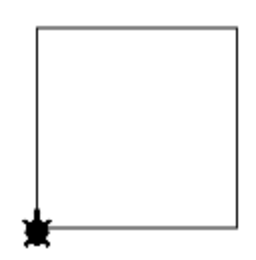
\includegraphics[width=0.35\linewidth]{GrundlagenInfo/00_Programmieren/Figures/quadrat}
\end{figure}
\end{column}
\begin{column}[t]{.5\textwidth}
\begin{lstlisting}
from gturtle import *
makeTurtle()

!\only<1>{distanz = 100}\only<2->{\colorbox{CarnationPink}{distanz = 100}}!
repeat 4:
    fd(!\only<1>{distanz}\only<2->{\colorbox{CarnationPink}{distanz}}!)
    rt(90)
\end{lstlisting}
\only<2->{
\vspace{1cm}
$\rightarrow$  = \colorbox{CarnationPink}{Variable!}
}
\end{column}
\end{columns}
\end{frame}

\begin{frame}{Fazit}
\begin{itemize}
    \item Variablen sind Namen für Speicherplätze.
    \item Wir können jederzeit neue Variablen erstellen, z.B. \pythoninline{y=5} oder \pythoninline{x=10*3}
    \item Der im Speicherplatz abgelegte Wert kann verändert werden.
    \item Die Anweisung \pythoninline{x+=add} erhöht den Wert der Variable \pythoninline{x} um den Wert von \pythoninline{add}.
    \item Die Anweisungen: \pythoninline{-=}, \pythoninline{*=} und \pythoninline{/=}  funktionieren analog dazu.
\end{itemize}
\end{frame}

\begin{frame}{Übungen}
Allgemein: speichern Sie ihre Lösungen jeweils ab
\begin{itemize}
    \item \aufgabebox{Aufgaben 3.8, 3.9, 3.12, 3.13, 3.14, 3.17}
    \item \aufgabebox{Aufgaben 3.21, 3.23, 3.25, 3.26, 3.27, 3.29}
    \item \abgabebox{Abgabe (Moodle): Aufgabe 3.24}
    \item \abgabebox{Abgabe (Moodle): Aufgabe 3.30}
    \begin{itemize}
    \item Tipp: Nichts zeichnen, nur berechnen und mit \lstinline|print(...)| ausgeben!
    \end{itemize}
    \item \challengebox{Aufgabe 3.28}
\end{itemize}
\end{frame}